
\chapter{Implementation}\label{ch:implementation}
This project will utilize an approach that begins by identifying users, which include human and bot users, based solely on their mouse movement behavior~\cite{intrustion_detection_using_mouse_dynamics}.
Specifically, this project presents a user differentiation method based on mouse behavior metrics, such as movement angle, movement velocity, scroll velocity, etc., instead of relying on client IP addresses present in the server logs.
Further study could include metrics that are also used in previously implemented web bot detection schemes.
But this project will start with just the mouse behavior metrics.
The presented approach in this project implies that, upon identifying users based on their mouse use behavior, decisions to declare userX, which is a single cluster, as a human or a bot are reinforced by empirical evidence of web traffic patterns corresponding to userX.
This approach could be an improvement to the inaccuracies present in previous supervised learning-based web bot detection schemes.
Additionally, this "identify users first, then classify as human or bot" method is similar to the current industry standard of websites requiring all visitors to log into an account for further use of their website; which reinforces decisions to declare account-holderX as a human or a bot, regardless of the IP address of account-holderX.
However, this "log-in, then use website" method causes user friction~\cite{how_recaptcha_is_improving_user_experience}, a concept introduced and considered by the latest "covert" versions of reCAPTCHA, that implies the inconveniences a user must experience to prove they are human and not a bot.
An example of this could be requiring a user to click/check "I'm not a robot" on older versions of reCAPTCHA.
In conclusion, this project presents an unsupervised, clustering method to autonomously identify users, as if they were to log in to an account, providing a means to make more informed decisions of the "web bot-ness" of visitors on a website.

\section{Objective}\label{sec:objective}
The objective of this project is to present a novel approach for website administrators to detect web bots.
Supervised learning is a common ML approach to detect web bots.
In fact, most ML approaches to robot detection apply supervised learning~\cite{10.1145/3339252.3339267}.
This sort of approach consists of training a classifier, i.e.
a function mapping an input, which are usually feature vectors describing sessions, to an output, a session’s class labels, based on a training dataset, which includes labelled training samples.
The ability of the inferred function to determine correct class labels for new, unseen samples is assessed on a test dataset.
Many supervised learning techniques demonstrated their efficiency in classification of bots and humans, e.g., decision trees support vector machine, neural networks , and k-Nearest Neighbours.
All supervised learning approaches, however, share a common disadvantage, related to a difficulty with preparation of a reliable training dataset, in particular with assigning accurate class labels to sessions of camouflaged robots~\cite{ROVETTA2020102577}.
In conclusion, since web bots are increasing in sophistication, meaning they are behaving more like humans in terms of mouse and HTTP request behavior~\cite{10.1109/DSN.2013.6575366}~\cite{7371507}, obtaining accurate training data that represents such complex web bots has been an issue.
This, combined with the anonymity of proxies that scramble the IP addresses of web bots, has motivated this project.

\section{General Architecture}\label{sec:general-arcitecture}
The general architecture of this implementation is as follows:
\begin{enumerate}
    \item \textbf{data extraction}: The position metrics, timestamp and coordinates, of the user's mouse cursor are collected from the user's computer and sent to the server for analysis. The \textit{Dataset} section outlines this stage.
    \item \textbf{features generation}: From the inputted raw data recorded and sent from the user's machine, features that characterize the raw data, and the user's session pertaining to it, are generated. The \textit{Features Engineering} section outlines this stage.
    \item \textbf{features analysis}: Sessions are clustered based on the generated features. The \textit{Features Analysis} section outlines this stage.
    \item \textbf{classification}: Clusters of sessions are used to determine bottness of users at client IP addresses. The \textit{Classification} section outlines this stage, a stage anticipated for future work.
\end{enumerate}
\begin{center}
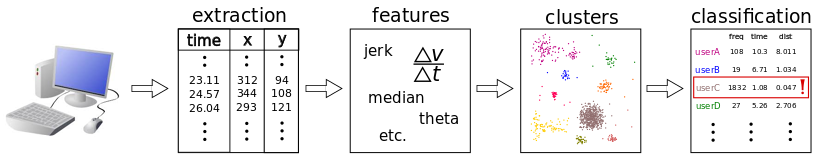
\includegraphics[width=1\columnwidth]{figures/general_architecture}
\end{center}

\section{Dataset}\label{sec:dataset}
In order to cluster users based on their mouse movement behavior, data of their mouse movement must be obtained.
An ideal scenario for this research would be to record the mouse movement of a high number of users, while navigating a specified user interface, thus creating a mouse movement recordings dataset.
But there are alternatives that maintain the validity of this research.

\subsection{Balabit Dataset}\label{subsec:balabit-dataset}
For testing and analysis purposes, a predefined dataset of users were used in this research.
The Balabit Mouse Challenge Dataset~\cite{balabit_dataset} was the primary dataset used in this research.
This dataset includes timing and positioning information of a web user's mouse pointer.
The authors of the dataset advertise that it can be used for authentication and identification purposes.
Researchers with focus on creating and evaluating the performance of behavioral biometric algorithms, which in this case draws from the mouse movement metrics of a user, are an intended audience for this publicly accessible dataset.
Originating from a data science competition on datapallet.io, the dataset is helpful to researchers and experts in the fields of IT security and datascience.

The competition for which the Balabit dataset originates from included a challenge of protecting users from unauthorized accesses into their accounts.
When users would login to their account, located on a remote server, recording their mouse movement behavior was a necessary step in an effort to increase account security.
Supposing that the method for which a user moves their mouse was unique to that user, a sort of biometric identifier can be obtained for account user authenticity.
If the mouse movement characteristics of a user, in a particular session, does not match the recorded and expected characteristics of the account holder, than that user in the particular session is said to be an unauthorized accessor.
In order to apply such a intrusion detection schema, a supervised learning-based model would need to be built and utilized.
However, this research does not intend on detecting unauthorized accessors, nor does it intend on using supervised learning in its implementation.

Although the Balabit dataset was intended to be used for creating and evaluating supervised learning-based models, the dataset still contains valuable user profiles and session recordings.
These user profiles are defined by a series of session recordings that are labeled with a single user of an account.
There are about 100 to 200 sessions recordings, spread over 10 users, with an average of 15 minutes of recording time per session.
Session recordings are split into two sets: training and testing.
This is for supervised learning uses.
For this research, all session files were combined into one set that is to be clustered and analyzed.
A session record is a csv file containing these fields~\cite{balabit_dataset}:
\begin{itemize}
    \item \textbf{record timestamp}: elapsed time (in seconds) since the start of the session as recorded by the network monitoring device used in the creation of the Balabit dataset
    \item \textbf{client timestamp}: elapsed time (in seconds) since the start of the session as recorded by the RDP client used by each of the 10 users
    \item \textbf{button}: the current condition of the mouse buttons
    \item \textbf{state}: additional information about the current state of the mouse
    \item \textbf{x}: the x coordinate (in pixels) of the mouse cursor on the screen
    \item \textbf{y}: the y coordinate (in pixels) of the mouse cursor on the screen
\end{itemize}
An example of a session record looks like:
\begin{center}
    \begin{tabular}{ |c|c|c|c|c|c| }
        \hline
        \textbf{record timestamp} & \textbf{client timestamp} & \textbf{button} & \textbf{state} & \textbf{x} & \textbf{y} \\
        \hline
        0.0 & 0.0 & NoButton & Move & 399 & 962 \\
        0.157999992371 & 0.155999999959 & NoButton & Move & 402 & 962 \\
        0.365999937057 & 0.248999999953 & NoButton & Move & 407 & 962 \\
        0.365999937057 & 0.358000000007 & Left & Pressed & 430 & 962 \\
        0.476999998093 & 0.467999999993 & Left & Released & 474 & 963 \\
        \ldots & \ldots & \ldots & \ldots & \ldots & \ldots \\
        \hline
    \end{tabular}
\end{center}
%duplicate session_0335985747

\subsection{Realtime Dataset}\label{subsec:realtime-dataset}
In a realtime environment, where the user differentiating algorithm is deployed, mouse movement data would come from the browser on the user's computer.
By using JavaScript's mousemove event listener, the coordinates of a user's mouse can be determined and recorded while a user is in session.
On average, a computers mouse position is polled 125 times per second~\cite{mouse_dpi_and_polling_rate_explained}~\cite{mouse_dpi_and_usb_polling_rate}.
This means that if a 10 second user session is recorded, there should be an average of 1,250 mouse position records of any single user browsing a website.
Records can be in a csv format:
\begin{itemize}
    \item \textbf{time}: elapsed time (in seconds) since the start of the session as recorded by the user's browser
    \item \textbf{x}: the x coordinate (in pixels) of the mouse cursor on the screen
    \item \textbf{y}: the y coordinate (in pixels) of the mouse cursor on the screen
\end{itemize}
A typical recorded session of a user's mouse movement metrics would look like:
\begin{center}
    \begin{tabular}{ |c|c|c| }
        \hline
        \textbf{time} & \textbf{x} & \textbf{y} \\
        \hline
        0.0 & 241 & 93 \\
        0.008121 & 278 & 77 \\
        0.015828 & 291 & 54 \\
        0.026942 & 302 & 48 \\
        0.037201 & 317 & 50 \\
        \ldots & \ldots & \ldots \\
        \hline
    \end{tabular}
\end{center}
These records can be stored on the user's computer, most likely in the browser via a JavaScript variable, then periodically sent to the server for which the website is hosted.
From this input, on the server, the web bot and botnet detection scheme will begin.
Pseudo code that generalizes the process of obtaining and sending a user's mouse movement metrics looks like:

{\color{darkgray} // the list of "times" "x" and "y" values POSTed to the server}
\newline
{\color{blue} \textbf{var}} records;

{\color{blue} \textbf{function}} flushRecords(bufSize)
\newline
\hspace*{25pt} {\color{darkgray} // reallocate "bufSize" number of indices for "times" "x" and "y" lists}

{\color{blue} \textbf{function}} postAndFlushRecords(bufSize)
\newline
\hspace*{25pt} {\color{darkgray} // POST all recorded "times" "x" and "y" values to the server}

{\color{blue} \textbf{function}} log(elapsedTime, x, y, bufSize)
\newline
\hspace*{25pt} {\color{darkgray} // insert "elapsedTime" "x" and "y" values into "records"}
\newline
\hspace*{25pt} {\color{darkgray} // postAndFlushRecords() if there are "bufSize" number of records}

{\color{blue} \textbf{function}} initBufferTimeout(timeLimit, bufSize)
\newline
\hspace*{25pt} {\color{darkgray} // postAndFlushRecords() every "timeLimit" duration}

{\color{blue} \textbf{function}} init()
\newline
\hspace*{25pt} {\color{darkgray} // use the "window" object's "onmousemove" func to log() mouse positions}
\newline
\hspace*{25pt} {\color{darkgray} // initBufferTimeout() to periodically POST logged "records" to the server}

{\color{darkgray} // called once upon every page load}
\newline
init();

The actual code, client{\_}mouse{\_}tracker.js, can be found in the src/ dir on the remote repo~\cite{thesis_github_repo} of this research.

\section{Features Engineering}\label{sec:features-engineering}
The intrustion detection scheme~\cite{intrustion_detection_using_mouse_dynamics}, while also using the Balabit dataset as it was intended to be used, extracted a set of features from the raw mouse position data.
Though their work implemented a supervised learning-based binary classifier, the features they extracted were proven to be effective metrics in differentiating and identifying users.
Instead of using all 6 elements of a datapoint vector, as outlined in the \textit{Balabit Dataset} section, we elected to only use the client timestamp ($t$), x position ($x$), and y position ($y$) values.
These three values construct a triplet, ($t_i$, $x_i$, $y_i$), $i = 1{\dots}n$, where $n$ is the number of recorded mouse positions, or datapoint vectors, in a session file.
From these three values, or triplets, of a single datapoint vector, in the list of vectors of a session file, the following features were extracted:
\begin{itemize}
    \item \textbf{velocity}: $v_i = \frac{\Delta p_i}{\Delta t_i}$, where $\Delta p_i = \lvert p_{i+1} - p_i \rvert$ and $\Delta t_i = t_{i+1} - t_i$
    \item \textbf{horizontal velocity}: ${v_x}_i = \frac{\Delta x_i}{\Delta t_i}$, where $\Delta x_i = \lvert x_{i+1} - x_i \rvert$ and $\Delta t_i = t_{i+1} - t_i$
    \item \textbf{vertical velocity}: ${v_y}_i = \frac{\Delta y_i}{\Delta t_i}$, where $\Delta y_i = \lvert y_{i+1} - y_i \rvert$ and $\Delta t_i = t_{i+1} - t_i$
    \item \textbf{acceleration}: $a_i = \frac{\Delta v_i}{\Delta t_i}$, where $\Delta v_i = \lvert v_{i+1} - v_i \rvert$ and $\Delta t_i = t_{i+1} - t_i$
    \item \textbf{jerk}: $j_i = \frac{\Delta a_i}{\Delta t_i}$, where $\Delta a_i = \lvert a_{i+1} - a_i \rvert$ and $\Delta t_i = t_{i+1} - t_i$
    \item \textbf{theta}: $\Theta _i = \arctan 2(\frac{\Delta y_i}{\Delta x_i})$, where $\Delta y_i = \lvert y_{i+1} - y_i \rvert$ and $\Delta x_i = \lvert x_{i+1} - x_i \rvert$
\end{itemize}

\subsection{Realtime Generation}\label{subsec:realtime-generation}
As described in the objective, this implementation is meant to detect web bots and botnet attacks in realtime.
At this stage of the detection scheme, a program would need to be run in realtime to compute the 6 features outline above.
Initially, a Python program was used to generate these 6 features as described.
The program calculated all 1676 session files, from all 10 users, in an average of 7 minutes.
By pre-allocating lists of numeric values, and incrementing a counter variable that keeps track of where to insert the next calculated feature value into the list of numeric values, the runtime was reduced from 7 minutes to slightly more than 3 minutes.
Further, the entire features generator program was converted from Python to Golang.
By creating Go-routines on each of the 6 features, the average runtime of the Golang program calculating all 1676 sessions files was less than 30 seconds.
All runtimes for realtime feature generation do not include data cleaning and prep.
Since the Balabit dataset has many duplicate timestamp values, with different \textit{x} and \textit{y} values, a pre-generation step would need to take place to remove erooneous duplicates, as a means to "clean" the raw data input.

\subsection{Statistics}\label{subsec:statistics}
After the $n$ feature values have been generated, where $n$ is the number of datapoint vectors or triplets in a session, for each of the 6 features, the values would need to be represented with statistical values.
The statistical values used for each of the 6 features are \textbf{mean}, \textbf{median}, \textbf{mode}, \textbf{interquartile range}, \textbf{minimum}, \textbf{maximum}, \textbf{range}, and \textbf{standard deviation}.

It is worth noting that the \textit{mode} and \textit{minimum} values did not appear to be as useful as the other statistical metrics.
The minimum values of each of the feature values lists were mostly zero.
This is a result of the feature calculations.
For example, horizontal velocity could be zero if the $x$ position does not change in two successive datapoint vectors.
Formally, ${v_x}_i = \frac{\Delta x_i}{\Delta t_i} = 0$ if $\Delta x_i = \lvert x_i - x_{i+1} \rvert = 0$, meaning $x_i = x_{i+1}$.
This is one example of why the \textit{maximum} and \textit{range} values were often the same.
If $range = \vert maximum - minimum \rvert$, where $mimimum = 0$, than $range = maxmimum$.
